\section{Laboratory Lecture 5: Keypad Control}
\label{sec:KEYPAD_GENERAL}

The aim of this practice is to understand how shift registers work, how to impement them using VHDL and, finally, how to build a keypad-controlled 7-segment display using a ring counter, a specific application of shift registers. This knowledge will be later used to implement more complex systems in further laboratory sessions. 

\subsection{Introduction}

Before delving into the practice itself, we will first go over the basics of shift registers, counters, keypads, and 7-segment displays.

\subsubsection{Shift Registers}
\label{sec:SHIFT_REGISTERS}

A shift register can be described as an array of flip-flops (\textbf{See Section \ref{sec:FLIP_FLOPS} for more information on this topic}) in which the output of one of connected to the input of the next one. They are mostly used in applications that involve the storage and transfer of data in a digital system.\medskip

A \textbf{register} is a digital circuit with two basic functions: data storage and data movement.
The storage capability of a register makes it an important type of memory device. Figure \ref{fig:D_FLIP_FLOP} illustrates the concept of storing a 1 or a 0 in a D flip-flop. A 1 is applied to the data input as shown, and a clock pulse is applied that stores the 1 by \textit{setting} the flip-flop. When the 1 on the input is removed, the flip-flop remains in the \textit{SET} state, thereby storing the 1. A similar procedure applies to the storage of a 0 by \textit{resetting} the flip-flop, as also illustrated in Figure \ref{fig:D_FLIP_FLOP} ~\autocite{FLOYD}

\begin{figure}[H]
    \centering
    \hspace{0.88cm}
    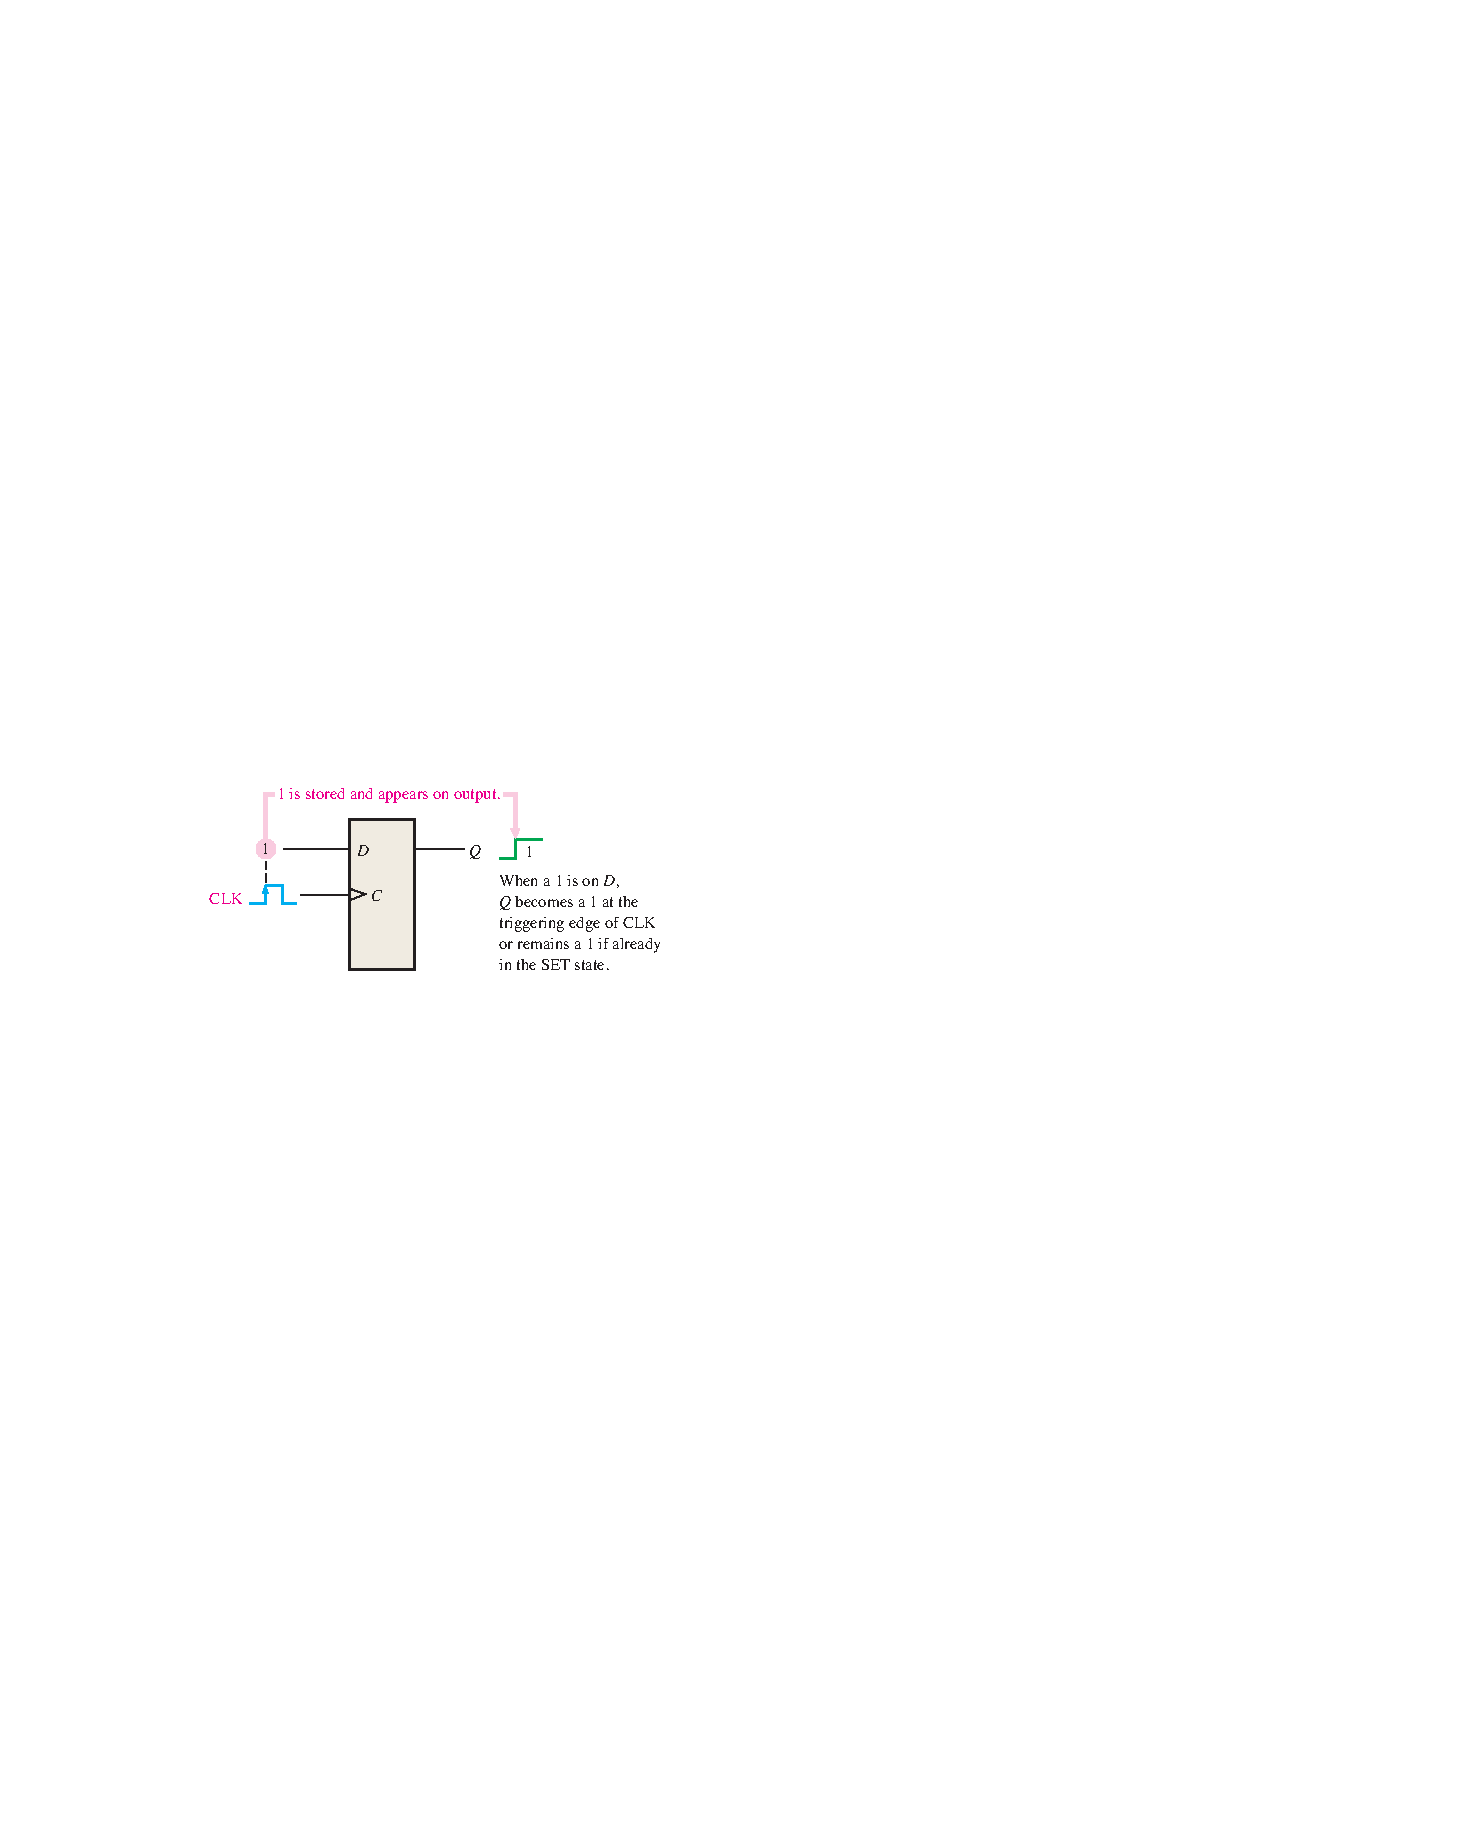
\includegraphics[scale = 1]{Graphics/VHDL/Practice 5/SHIFT_REGISTER_BASICS/D-Latch_Operation_451_1.pdf}
\end{figure}

\begin{figure}[H]
    \centering
    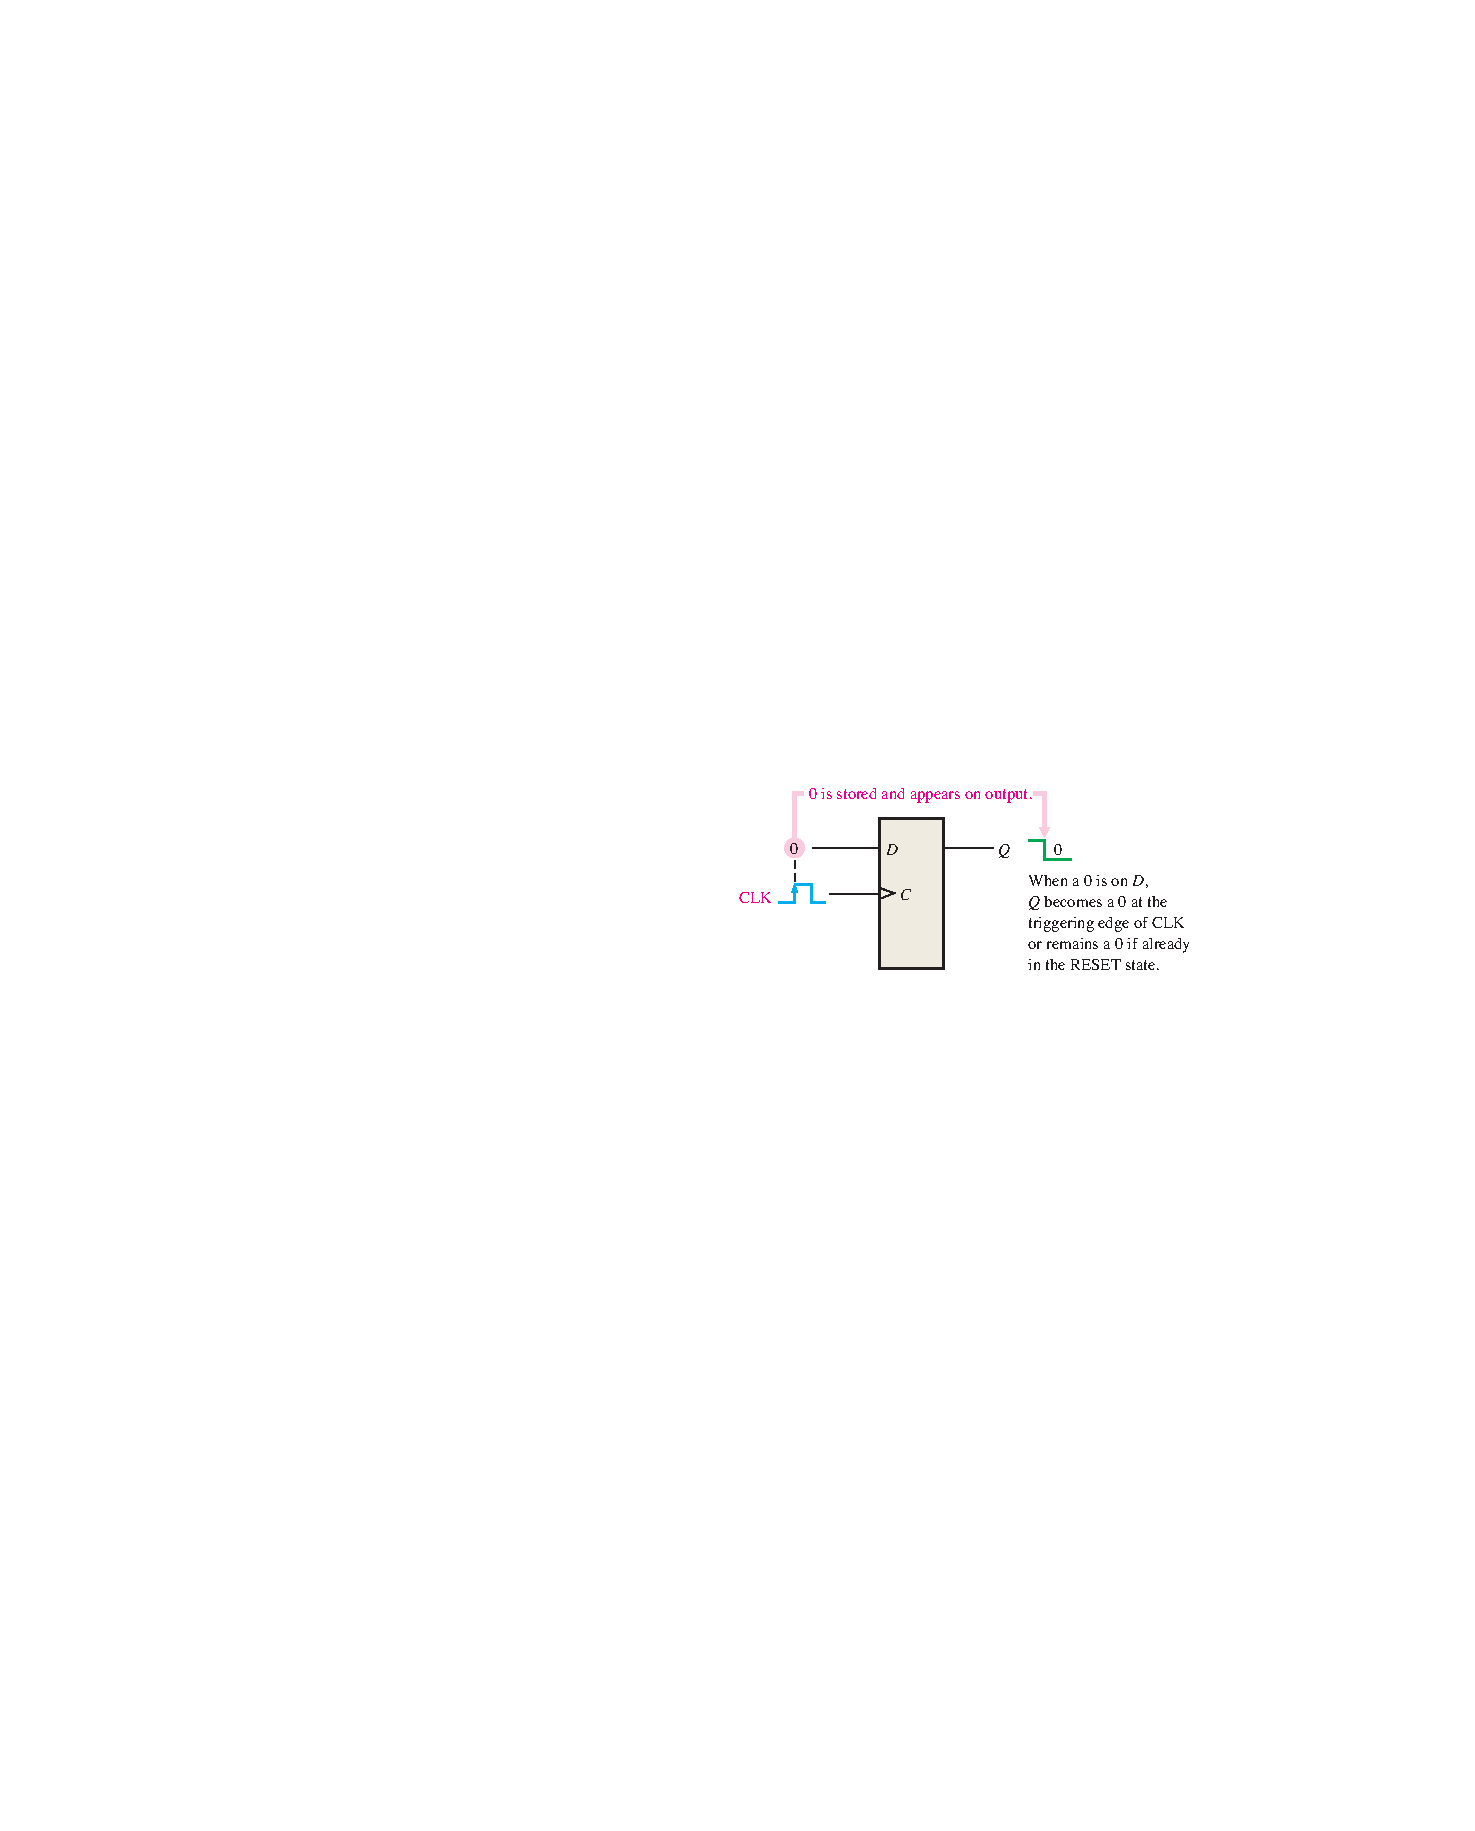
\includegraphics[scale = 1]{Graphics/VHDL/Practice 5/SHIFT_REGISTER_BASICS/D-Latch_Operation_451_2.pdf}
    \caption{D-Flip Flop as a data storage element ~\autocite{FLOYD}}
    \label{fig:D_FLIP_FLOP}
\end{figure}

\clearpage

Depending on the configuration of the flip-flops, the data that they trasmit and store can be \textit{shifted}, or moved, in several ways. We can see this in the illustration attached below:

\begin{figure}[H]
    \centering
    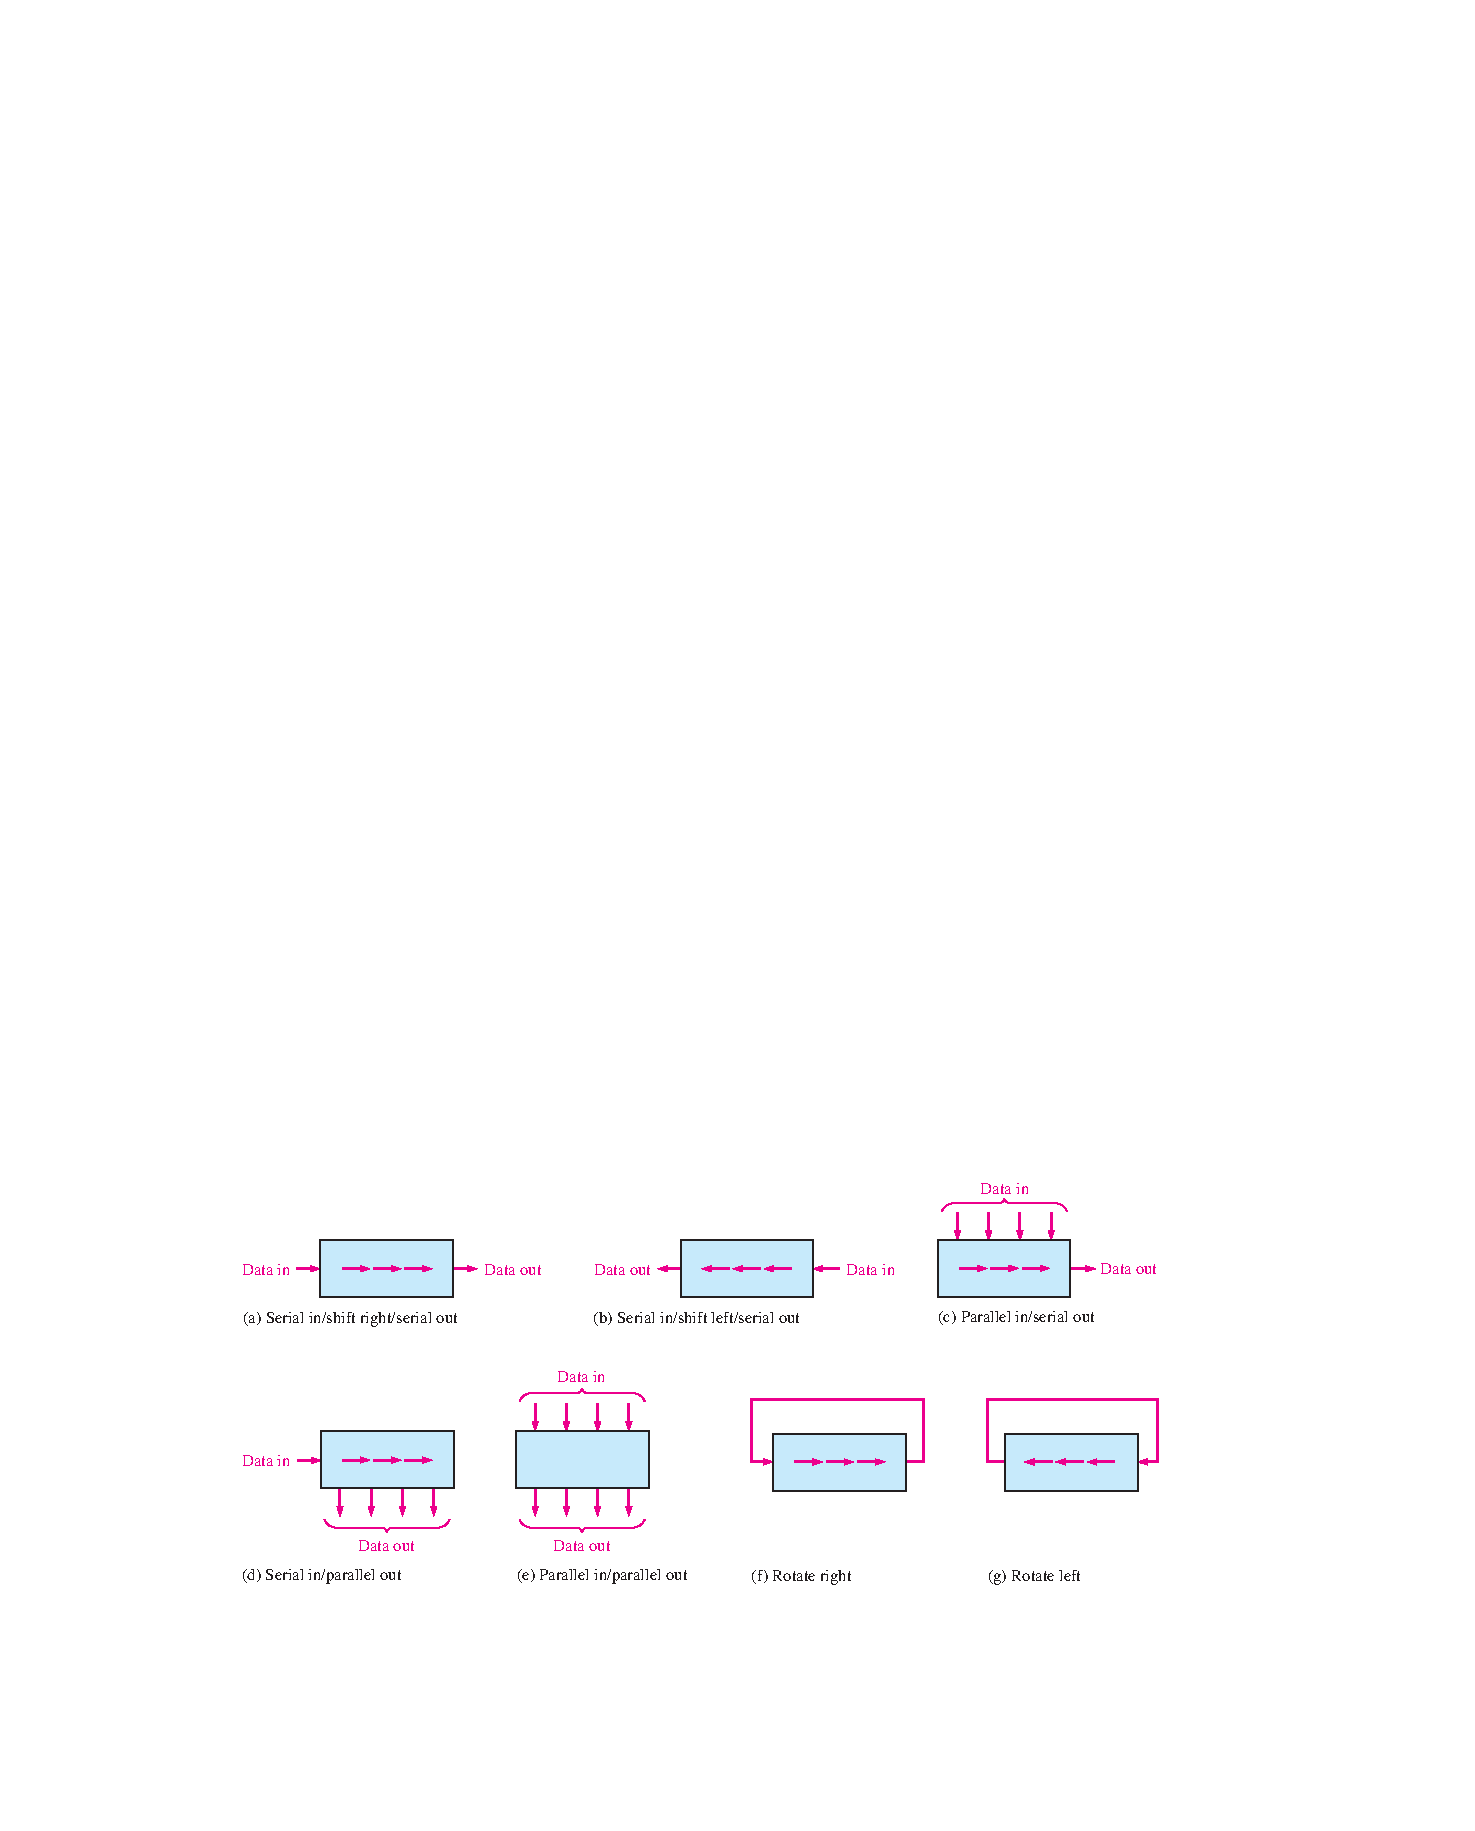
\includegraphics[scale = 0.85]{Graphics/VHDL/Practice 5/SHIFT_REGISTER_BASICS/DATA_TRANSMISSION/Data_Movement_451.pdf}
    \caption{Different types of data transfer ~\autocite{FLOYD}}
    \label{fig:DATA_TRANSFER}
\end{figure}

These different configurations allow us to streamline the transmission and storage of data. By using, for instance, a Parallel-In Serial-Out configuration, we can reduce the amount of wires that are needed to perform a data transmission. Even though a serial transmission is slower than a parallel one, one might argue that for most day to day applications, its speed is enough. Examples of this may include the USB bus, UART, SPI, and I2C communication and so on.\medskip

The opposite also exist, as we can see in Figure \ref{fig:DATA_TRANSFER}. In fact, it is common to use a combination of both transmission methods in order to transfer data reliably and cost effectively, since all of the data packets are transmitted using one wire instead of multiple ones. The only thing that the user must do to obtain the initial parallel data is to \textit{decode} the stream of serial data. To do this a Serial-In Parallel-Out shift register is used. \medskip

\clearpage

We can see an example of this type of data transfer below:

\begin{figure}[H]
    \centering
    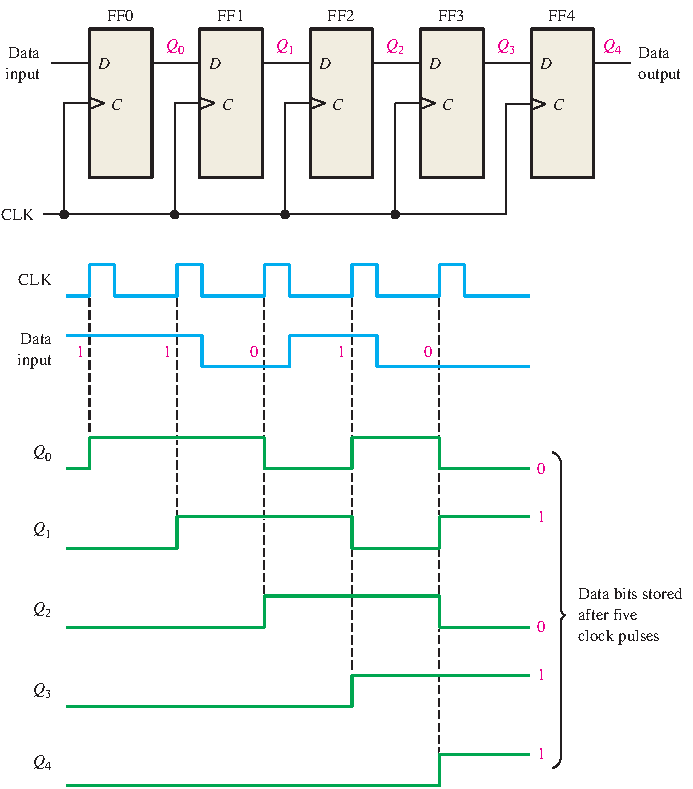
\includegraphics[]{Graphics/VHDL/Practice 5/SHIFT_REGISTER_BASICS/DATA_TRANSMISSION/SIPO_and_Wave.pdf}
    \caption{Serial-In Parallel-Out ~\autocite{FLOYD}}
    \label{fig:SIPO}
\end{figure}

As we can see in the picture, every time that there a PGT occurs, the data in the input in introduced in the first Flip-Flop and the rest of the data skips on place. In this example in particular, after 4 clock cycles, the 4 input data bits are shown in $Q_0 - Q_3$ at the same time, effectively converting serial data into parallel data.\medskip

\clearpage

\subsubsection{Counters}
\label{sec:COUNTERS}

On the other hand, shift registers can also be used to create \textbf{counters}. A shift register counter is basically a shift register with the serial output connected back to the serial input to produce special sequences. These devices are often classified as counters because they exhibit a specified sequence of states.\medskip 

Two of the most common types of shift register counters are the Johnson counter and the Ring counter. The main difference between them is the connection between the output of the last flip flop to the input of the first one. In Ring counters, the output \bm{$Q_{final}$} is directly connected to the input \bm{$D_{initial}$}, whereas in Johnson counters, the output that gets connected to the inpus is the \bm{$\overline{Q_{final}}$}. \medskip

Even though they are similar, these counters do not behave in the same way. One of the main disadvantages of ring counters is that thet must be preloaded with the desired pattern (usually a single 0 or 1). Besides, ring counters have even fewer states than Johnson ones (n, where $n = $ number of flip-flops). On the other hand, they have the advantage of being self-decoding, with a unique output for each state.\medskip

We can see examples of both of these counters below:

\begin{figure}[H]
    \centering
    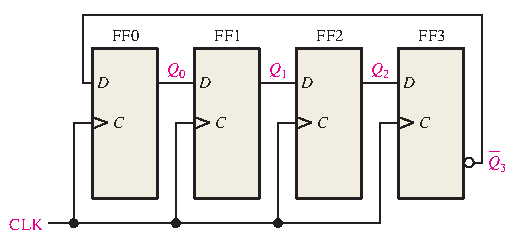
\includegraphics[scale = 0.8]{Graphics/VHDL/Practice 5/COUNTERS/Johnson_Counter_467.pdf}
    \caption{4-bit Johnson counter ~\autocite{FLOYD}}
    \label{fig:JOHNSON_4_BIT}
\end{figure}

\begin{figure}[H]
    \centering
    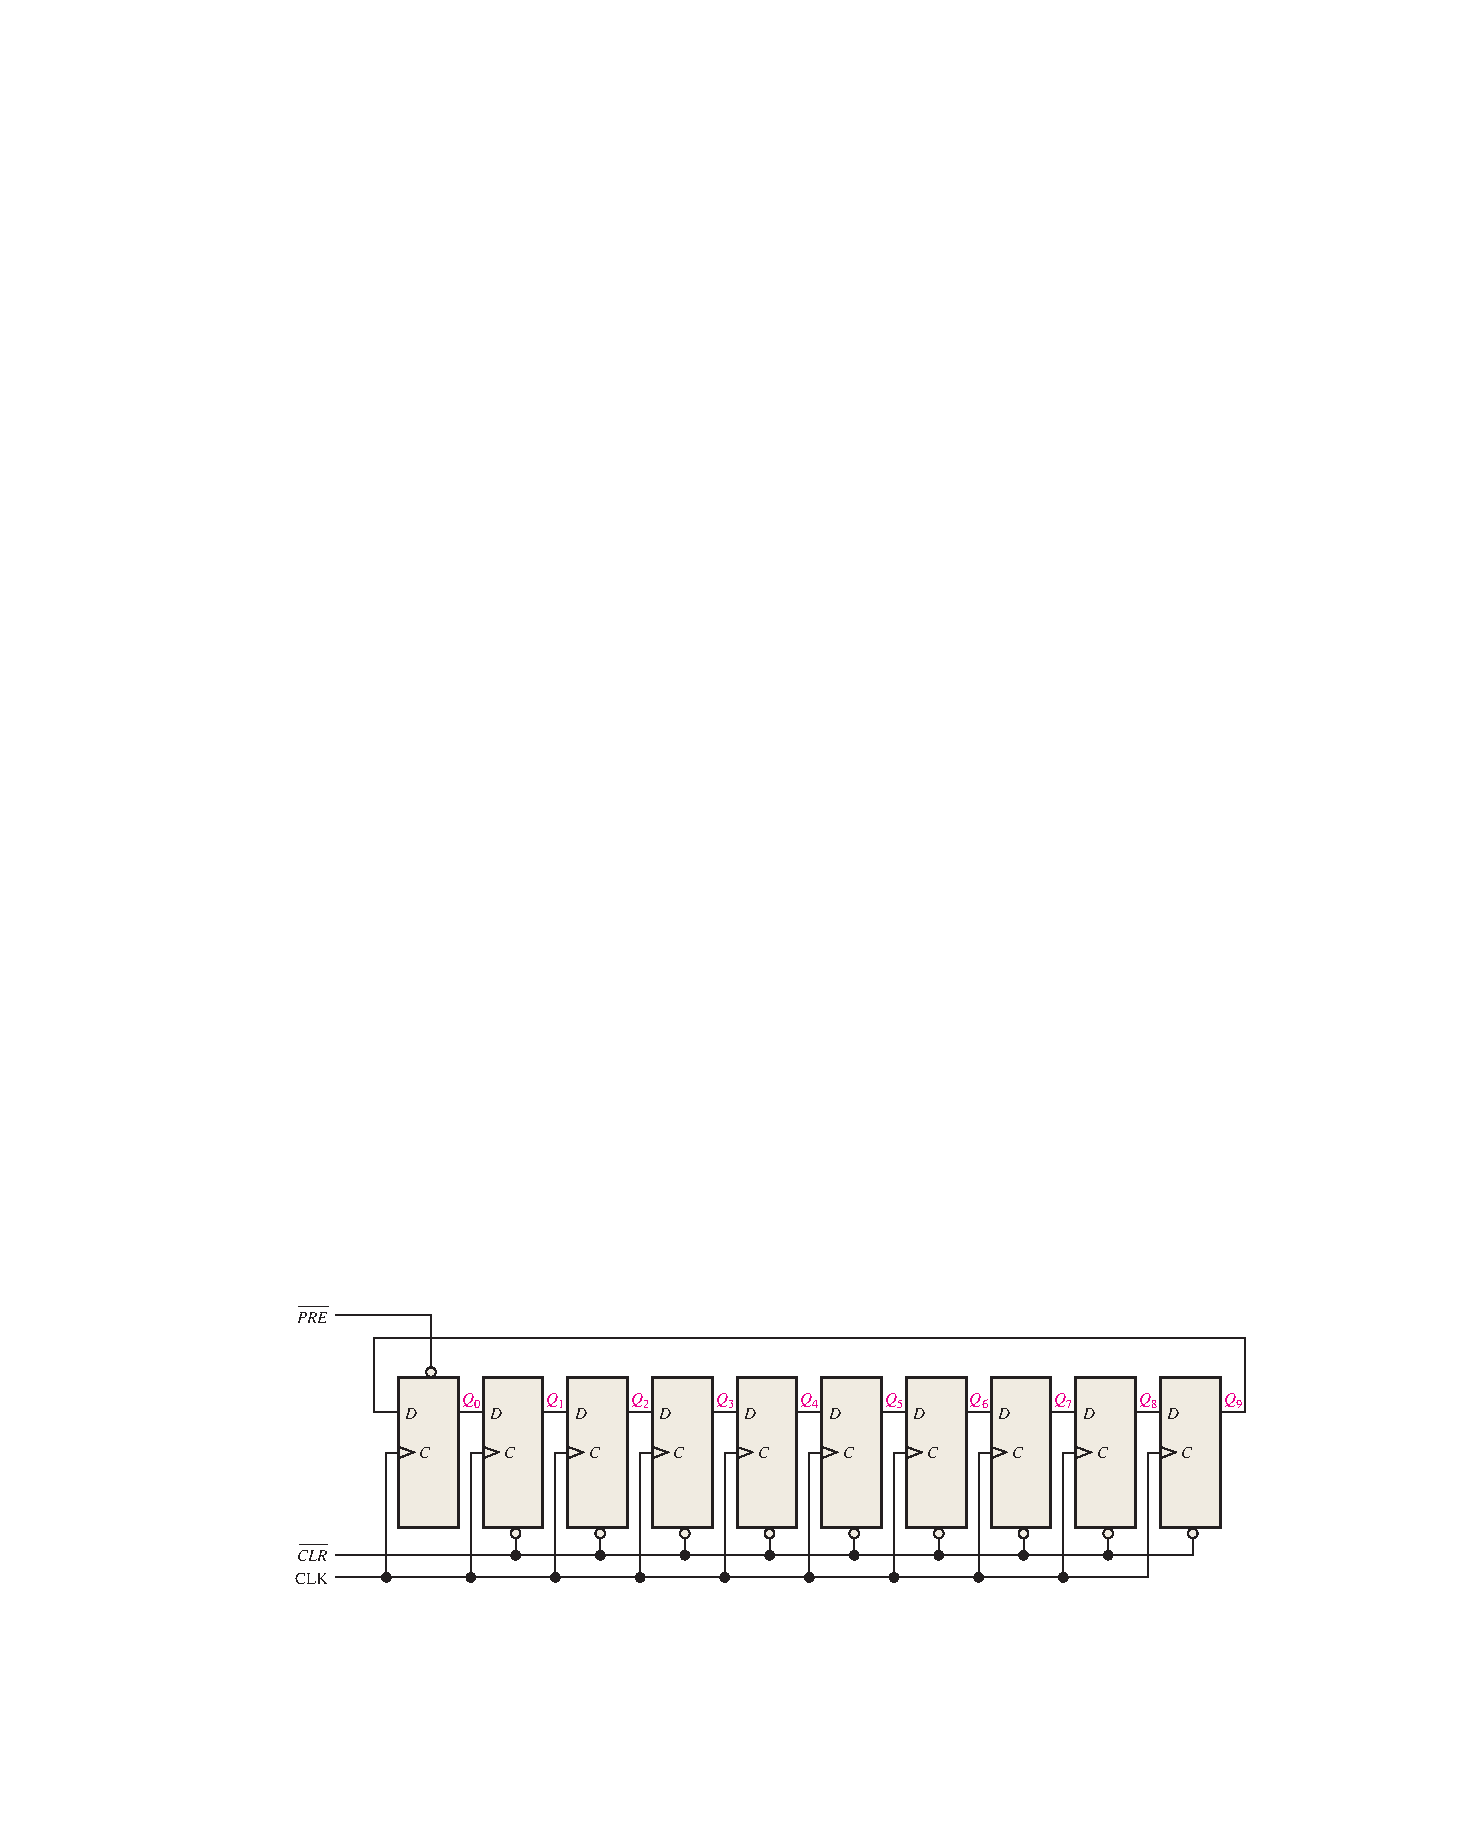
\includegraphics[scale = 0.8]{Graphics/VHDL/Practice 5/COUNTERS/RING_COUNTER.pdf}
    \caption{10-bit Ring counter ~\autocite{FLOYD}}
    \label{fig:RING_10bit}
\end{figure}

\clearpage

\subsubsection{Keypad}
\label{sec:KEYPAD}

In this laboratory practice we have used a 4x3 keypad as a HMI (Human-Machine Interface) so as to allow us to introduce different numbers in our system.\medskip

A keypad is no more than a bi-dimensional array of pushbuttons that are connected together in a matrix configuration in order to reduce the number of data lines that the user must use to read the different signals. We can see this array in the picture attached below:


\begin{figure}[H]
    \centering
    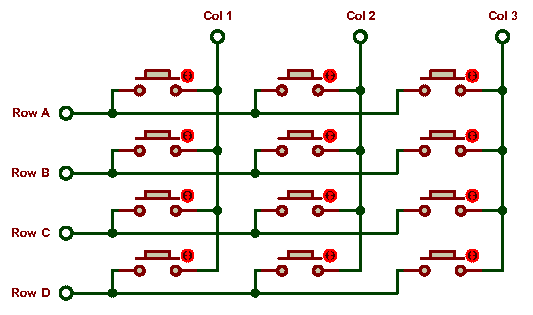
\includegraphics[scale = 1]{Graphics/VHDL/Practice 5/KEYPAD/KEYPAD_BUTTONS.PDF}
    \caption{3x4 Matrix Keypad Pushbutton Array}
    \label{fig:KEYPAD_BUTTON}
\end{figure}

Normally, a ring counter (\textbf{See Subsubsection \ref{sec:COUNTERS} for more on this topic}) is used to circulate a logic \textit{1} in the rows, allowing the CPU to detect which button has been pressed based on the both column in which a HIGH level has been detected and the position of the \textit{1} in the rows. We will dive into this later.\medskip

The proteus representation of this array of buttons can be seen below:\medskip


\begin{figure}[H]
    \centering
    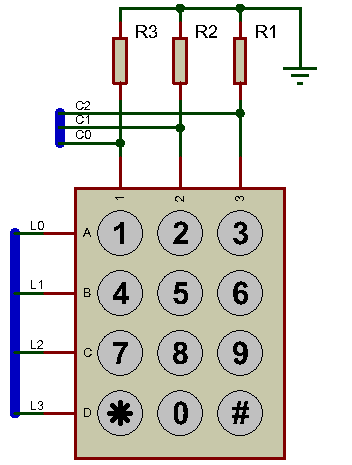
\includegraphics[scale = 0.85]{Graphics/VHDL/Practice 5/KEYPAD/KEYPAD.PDF}
    \caption{Proteus built-in keypad}
    \label{fig:PROTEUS_KEYPAD}
\end{figure}

\clearpage

\subsubsection{7-segment Displays}
\label{sec:7_SEG_DISP}

A 7-segment display can be described as a module composed of an array of LEDs which are arranged in a special way that enables the user to display different numbers and letters. In this practice we will use them to show the number that the user has entered.\medskip

\begin{figure}[H]
    \centering
    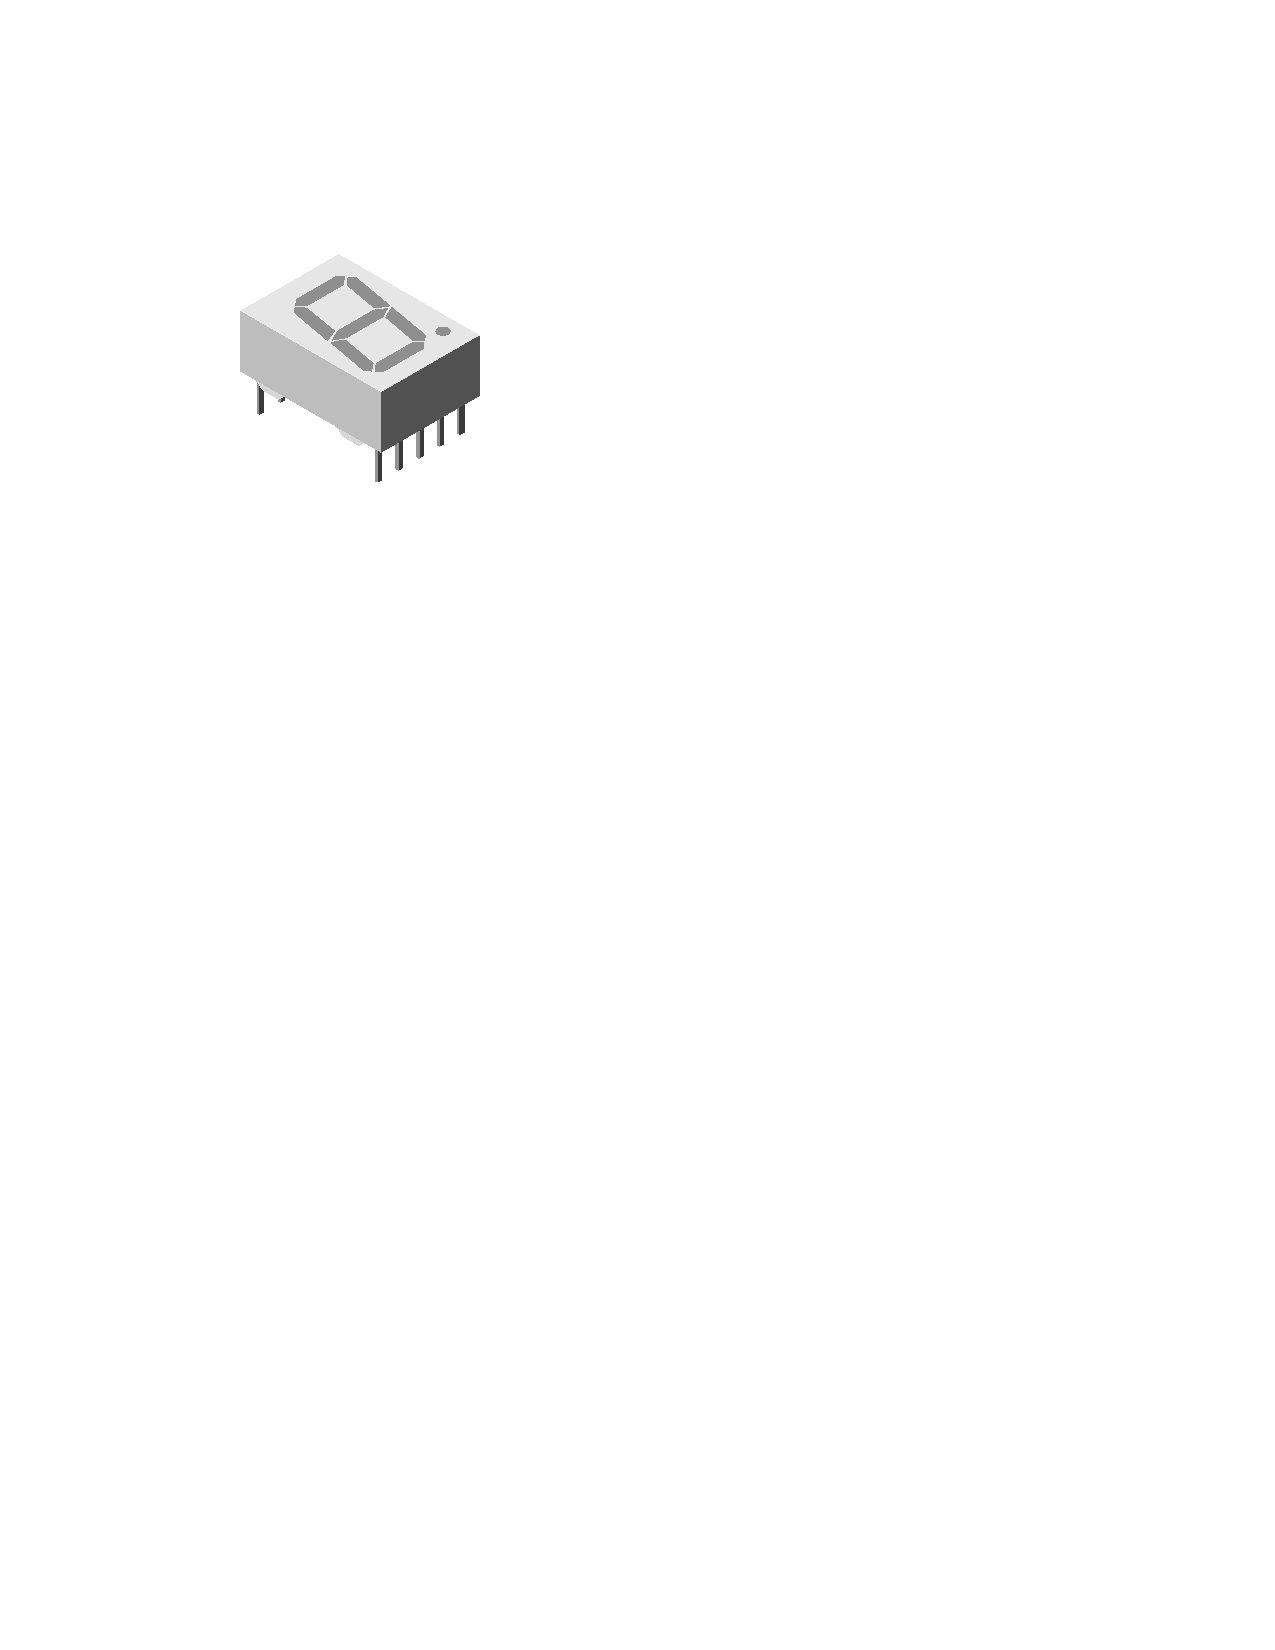
\includegraphics[scale = 0.9]{Graphics/VHDL/Practice 5/7-SEG/3D_MODEL.pdf}
    \caption{3D Model of a 7-Segment display ~\autocite{7-SEGMENT}}
    \label{fig:7-SEG-3D}
\end{figure}

As its name suggests, there are 7 of these LEDs, or segments, plus a decimal point, that may be used to indicate the magnitude of a floating point number. We can see these segments in the following image: \medskip

\begin{figure}[H]
    \centering
    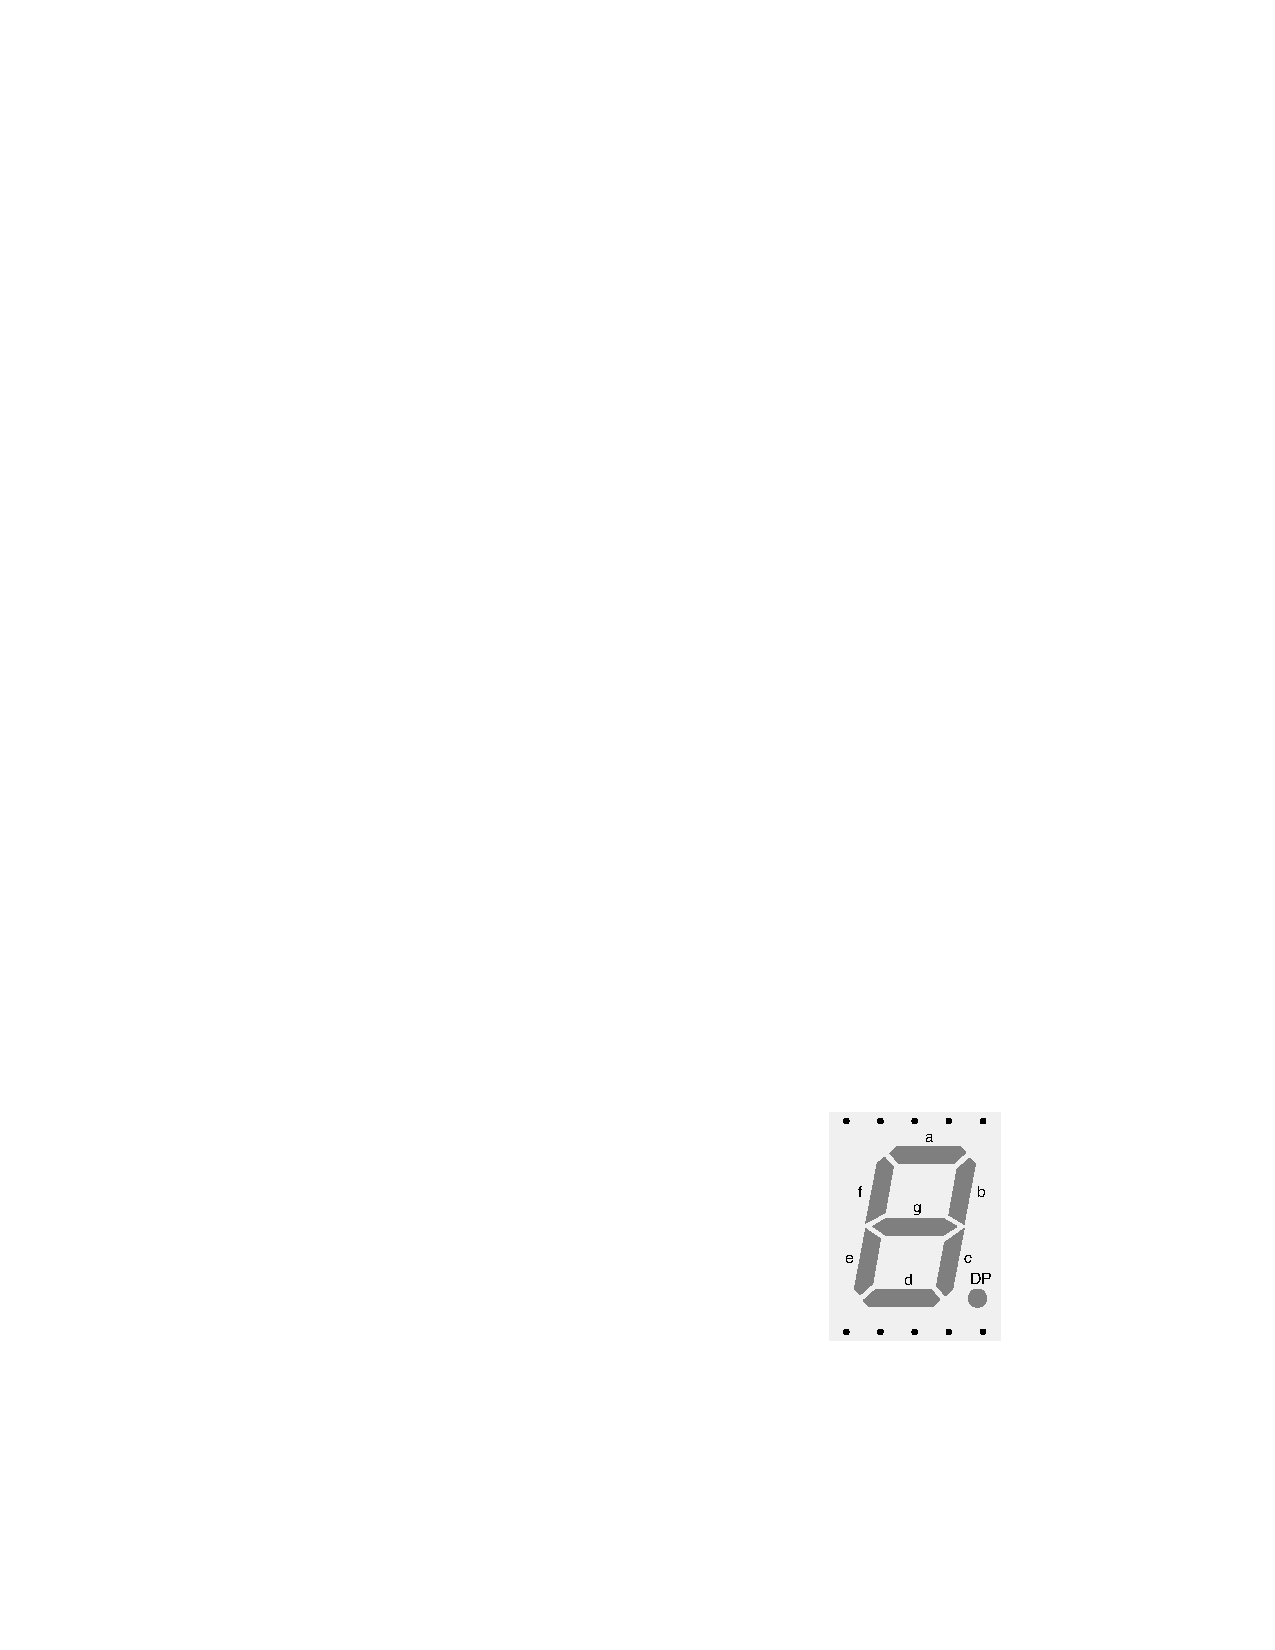
\includegraphics[]{Graphics/VHDL/Practice 5/7-SEG/SEGMENTS.pdf}
    \caption{7-Segment Display individual segments ~\autocite{7-SEGMENT}}
    \label{fig:7-SEG-SEGMENTS}
\end{figure}

\clearpage

Now that we have established how the different elements that make up our circuit work and behave, we will move on to solving the proposed exercises.

\subsection{Exercise 1: Ring Counter with 74HC194}

As we have seen in Subsubsection \ref{sec:COUNTERS}, Ring Counters can be built using Shift Registers, which, in essence, are just multiple Flip-Flops tied together (\textbf{Subsection \ref{sec:FLIP_FLOPS}}). Readily available, off-the-shelf ICs that integrate these kind of counters exist as well. One example of said ICs would be the \textbf{74HC194}. \medskip

\subsubsection{General Description}

The \textbf{74HC194} is a 4-bit bidirectional universal shift register which truth table can be seen below: \medskip

\begin{table}[htbp]
    \resizebox{\columnwidth}{!}{
        \centering
        \begin{tabular}[t]{lccccccccccccc}
            \toprule
            & \textbf{Operating Mode} \vspace{0.2cm} & &\multicolumn{7}{c}{\textbf{Inputs \; \; \; \; \;}} & \multicolumn{4}{c}{\textbf{Outputs}}\\
            
            & & \textbf{CP} & $\mathbf{\overline{MR}}$ & $\mathbf{S_1}$ & $\mathbf{S_0}$ & \textbf{DSR} & \textbf{DSL} & $\mathbf{D_n}$ & & $\mathbf{Q_0}$ & $\mathbf{Q_1}$ & $\mathbf{Q_2}$ & $\mathbf{Q_3}$\\
             
            \midrule
            & \textbf{Reset (clear)} & X & L & X & X & X & X & X & & L & L & L & L\\
            \midrule
            & \textbf{Hold (do nothing)} & X & H & l & l & X & X & X & & q0 & q1 & q2 & q3\\
            \midrule
            & \textbf{Shift Left} & $\uparrow$ & H & h & l & X & l & X & & q1 & q2 & q3 & L\\
            & & $\uparrow$ & H & h & l & X & h & X & & q1 & q2 & q3 & H\\
            \midrule
            & \textbf{Shift Right} & $\uparrow$ & H & l & h & l & X & X & & L & q0 & q1 & q2\\
            & & $\uparrow$ & H & l & h & h & X & X & & H & q0 & q1 & q2\\
            \midrule
            & \textbf{Parallel Load} & $\uparrow$ & H & h & h & X & X & dn & & d0 & d1 & d2 & d3\\
            \bottomrule
        \end{tabular}
        \caption{Functional description of 74HC194 ~\autocite{74HC194}}
        \label{table:74HC194}
        }
\end{table}

The synchronous operation of the device is determined by the mode select inputs ($\mathit{S_0}$, $\mathit{S_1}$). In parallel load mode ($\mathit{S_0}$ and $\mathit{S_1}$ HIGH) data appearing on the $\mathit{D_0}$ to $\mathit{D_3}$ inputs, is transferred to the $\mathit{Q_0}$ to $\mathit{Q_3}$ outputs. When $\mathit{S_0}$ is HIGH and $\mathit{S_1}$ is LOW data is entered serially via \textit{DSL} and shifted from left to right; when $\mathit{S_0}$ is LOW and $\mathit{S_1}$ is HIGH data is entered serially via \textit{DSR} and shifted from right to left. \textit{DSR} and \textit{DSL} allow multistage shift right or shift left data transfers without interfering with parallel load operation. If both $\mathit{S_0}$ and $\mathit{S_1}$ are LOW, existing data is retained in a hold mode. Mode select and data inputs are edge-triggered, responding only to the LOW-to-HIGH transition of the clock (\textit{CP}). Therefore, the only timing restriction is that the mode control and selected data inputs must be stable one set-up time prior to the positive transition of the clock pulse. When LOW, the asynchronous master reset (\textit{MR}) overrides all other input conditions and forces the \textit{Q} outputs LOW. ~\autocite{74HC194}

\clearpage

\subsubsection{Application: Ring Counter}

The aim of the first part of the laboratory lecture is to build a \textbf{ring counter} using a 74HC194. In order to do this, we will follow the following sequence:

\begin{enumerate}
    \item Reset
    \item Parallel Load ($D_n$ = 0100)
    \item Shift Left / Right
\end{enumerate}

This rather simple circuit circuit will allow us to visualize the behaviour of ring counters. We will use ISIS Proteus to perform the simulation:

\begin{figure}[H]
    \centering
 
    \ifnum\value{ANIMATION}=1 {
        \animategraphics[controls,loop,scale=1.1]{1}{Graphics/VHDL/Practice 5/74HC194/ORIGINAL/F}{0}{5}
    } 
    \else {
        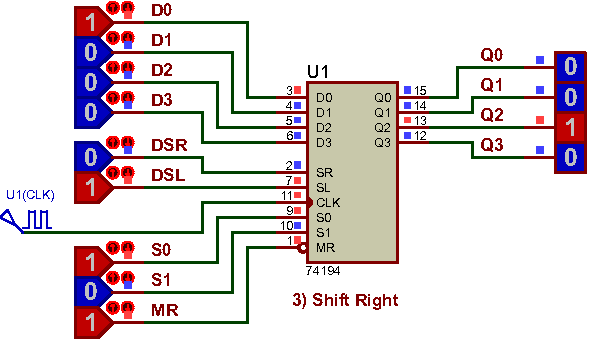
\includegraphics[scale=1.1]{Graphics/VHDL/Practice 5/74HC194/ORIGINAL/F4.PDF}
    }\fi
    
    \caption{Basic Shift Right Operation}
    \label{fig:74HC194_SHIFT_RIGHT}
\end{figure}

As we have seen, the 74HC194 is not a counter but a shift register, which means that once we preload the \textit{1} and we let it run, after just 4 clock cycles, the outputs $Q_n$ will return to \textit{0000}. In other words, the \textit{1} will be shifted right 4 times, and its previous position will be replaced by a \textit{0}, effectively resetting the register.\medskip

To solve this issue, we will connect $Q_3$ back to the \textit{DSR} pin so that when the \textit{1} gets to the last position, the counter preloads itself with \textit{1000} and starts again.\medskip

To control the counter, we will make use of the two selection pins $S_0$ and $S_1$. As we can see in Table \ref{table:74HC194}, when $S_0 = 1$ and $S_1 = 1$, the inputs $D_n$ will be loaded in the output $Q$, and when $S_0 = 1$ and $S_1 = 0$, provided that $DSR = 0$, the counter will start right-shifting the preloaded \textit{1} bit. Once the \textit{1} gets to $Q_3$, the $DSR$ pin will be pulled HIGH and, in the next cycle, the counter will introduce a \textit{1} in $Q_0$ instead of a \textit{0}. This keeps the counter going until the S pins are pulled HIGH, in which case the operation would be halted and the counter would be restarted back to the original state.\medskip

We can see this in the following animation:

\begin{figure}[H]
    \centering
 
    \ifnum\value{ANIMATION}=1 {
        \animategraphics[controls,loop,scale=1.1]{1}{Graphics/VHDL/Practice 5/74HC194/MODIFIED/F}{0}{9}
    } 
    \else {
        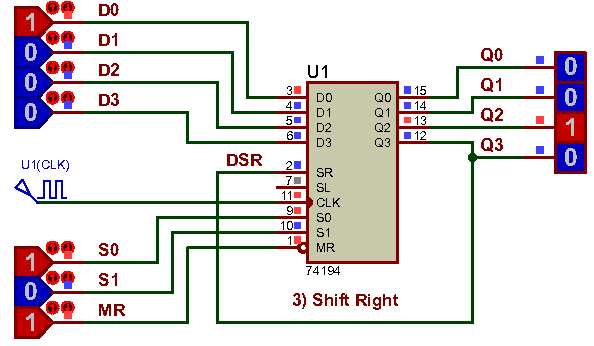
\includegraphics[scale=1.1]{Graphics/VHDL/Practice 5/74HC194/MODIFIED/F4.PDF}
    }\fi
    
    \caption{Ring Counter with 74HC194}
    \label{fig:74HC194_RING}
\end{figure}

\clearpage 

\subsection{Exercise 2: Ring Counter with VHDL}
\label{sec:RING_VHDL}

In this exercise we are asked to implement a ring counter such as the one seen in the previous exercise, but this time using VHDL and a GAL.\medskip

This GAL will include the following I/O:

\begin{itemize}
    \item \textbf{IR} as the synchronous control INPUT.
    \item \textbf{CLK} as the clock INPUT.
    \item $\mathbf{L\left[ 3...0 \right]}$ as the 4 OUTPUTS ($\mathbf{Q_n}$). 
\end{itemize}

The control input, \textit{IR} will operate as folows:

\begin{enumerate}
    \item If a HIGH is detected in this pin, \textit{0001} will be preloaded in the counter.
    \item Once the pin in pulled LOW, the ring counter will be started and it will continue until IR is pulled HIGH again. 
\end{enumerate}

To illustrate this behaviour, a flow diagram has been attached below:

\begin{figure}[H]
    \centering
    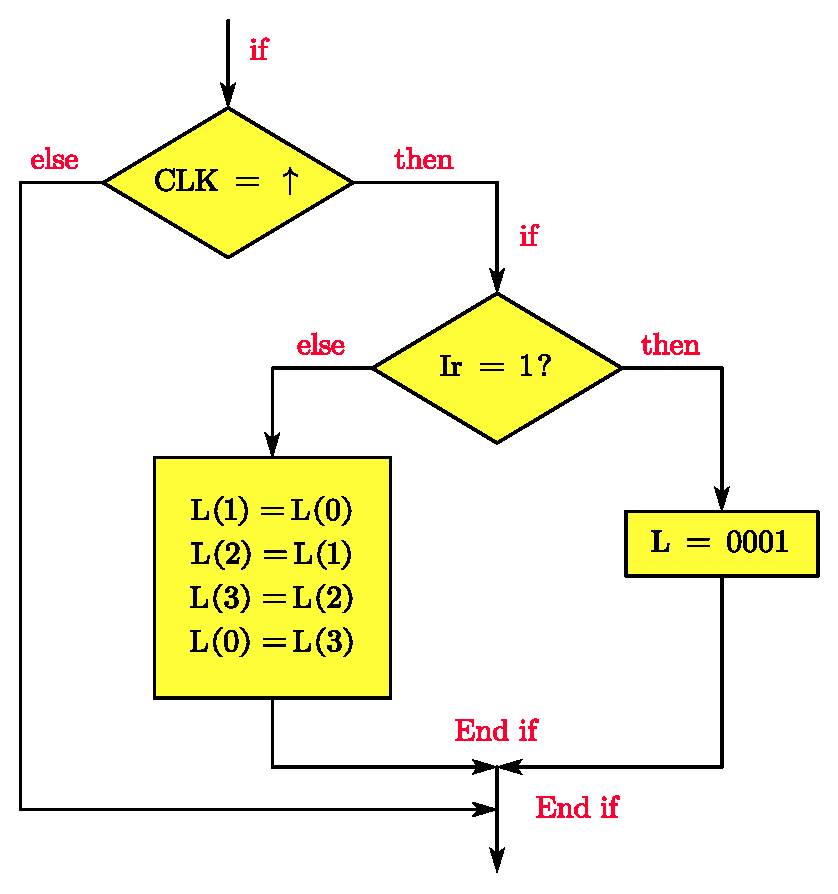
\includegraphics[scale = 0.7]{Graphics/VHDL/Practice 5/AXGLYPH/Block_Diagram.pdf}
    \caption{VHDL Ring Counter Flow Diagram}
    \label{fig:VHDL_RING_FLOW}
\end{figure}

\clearpage

The VHDL code that describes this process can be seen below:

\inputcode{CODES/VHDL/Practice_5/RING_COUNTER.vhd}

As we can see, a signal \textit{l\_temp} has been created so as to avoid modifying the outputs directly, as this may cause unwanted results.

\clearpage

\subsection{Exercise 3: 3x4 Keypad Control with VHDL}
\label{sec:KEYPAD_CONTROL_VHDL}

This exercise sums up all of the knowledge that we have aquired about different components such as shift registers, counters, 7-segment displays, and so on. \medskip

The aim of this last part is to create a system that displays what the user introduces via a keypad in a 7-segment display. To do this, we will make use of the VHDL ring counter that we have just seen in Subsection \ref{sec:RING_VHDL} to interface the keyboard and we will write what we read back to a BCD to 7-segment dislay driver, which, as the name suggests, will convert the output of the GAL, in BCD, to a readable decimal form in the 7-segment display.\medskip

To interface the keyboard we must use a ring counter so as to reduce the amount of needed pins. Otherwise, the GAL would most probably not be able to read all of the required inputs. For this particular case, a ring counter is used to circulate a logic 1 in the display's rows, allowing the GAL to detect which button has been pressed based on the both column in which a HIGH level has been detected and the position of the 1 in the rows, as seen in \textbf{Subsubsection \ref{sec:KEYPAD}}.\medskip

This GAL will include the following \textbf{inputs}:

\begin{itemize}
    \item \textbf{IR} as the synchronous control.
    \item \textbf{CLK} as the clock.
    \item $\mathbf{C\left[ 2...0 \right]}$ as the logic levels from Keypad columns. They are pulled LOW by default due to the pull-down.
\end{itemize}

Regarding the \textbf{outputs}, we find:

\begin{itemize}
    \item $\mathbf{L\left[ 3...0 \right]}$ as the ring counter outputs. 
    \item $\mathbf{Q\left[ 3...0 \right]}$ as the BCD Code corresponding to the pushed button, as shown the truth table below. 
\end{itemize}


\begin{table}[H]
    \centering
        \begin{tabular}[t]{lcccc}
            \toprule
            &\textbf{L3..L0}&\textbf{C2...C0}&\textbf{Button}&\textbf{BCD code}\\
            \midrule
                &    0001   & 001     & 1      & 0001     \\
                &    0010   & 001     & 4      & 0100     \\
                &    0100   & 001     & 7      & 0111     \\
                &    1000   & 001     & *      & 1100     \\
                &    0001   & 010     & 2      & 0010     \\
                &    0010   & 010     & 5      & 0101     \\
                &    0100   & 010     & 8      & 1000     \\
                &    1000   & 010     & 0      & 0000     \\
                &    0001   & 100     & 3      & 0011     \\
                &    0010   & 100     & 6      & 0110     \\
                &    0100   & 100     & 9      & 1001     \\
                &    1000   & 100     & \#     & 1111     \\
            \bottomrule
        \end{tabular}
        \caption{Reading to Button Conversion table ~\autocite{SLIDES_5}}
        \label{table: KEYPAD_TABLE}
\end{table}


The VHDL code that describes this process can be seen below:

\inputcode{CODES/VHDL/Practice_5/KEYPAD.vhd}

As we explained in Exercise 2 (\textbf{Section \ref{sec:RING_VHDL}}) this code is composed of a ring counter, which is initialized by the \textit{IR} pin, and the rest of the logic. We will not delve into the ring counter part again as it has already been explained before. \medskip

\clearpage

The rest of the code reads the button presses, interprets them and outputs the corresponding BCD code. To do this, we first start the ring counter, which is connected to the L terminals of the keypad. At the same time, we monitor the C lines of said keypad using the output \textit{pulse}. If pulse is pulled HIGH, meaning that one of the buttons has been pressed, we check both the pin of the C array in which the HIGH has been detected as well as the position of the one in the ring counter. Since there can only be one possible combination, i.e., only one row and one column can be active at the same time, the pressed button can be read using this method.\medskip

Once the pressed button has been determined, the GAL outputs its corresponding BCD code in $Q_n$. This output is connected through a BCD to 7-segment converter to the display. \medskip

We can see this here:

\begin{figure}[H]
    \centering
 
    \ifnum\value{ANIMATION}=1 {
        \animategraphics[controls,loop,scale=0.8]{1}{Graphics/VHDL/Practice 5/7-SEG/ANIMATION/F}{0}{9}
    } 
    \else {
        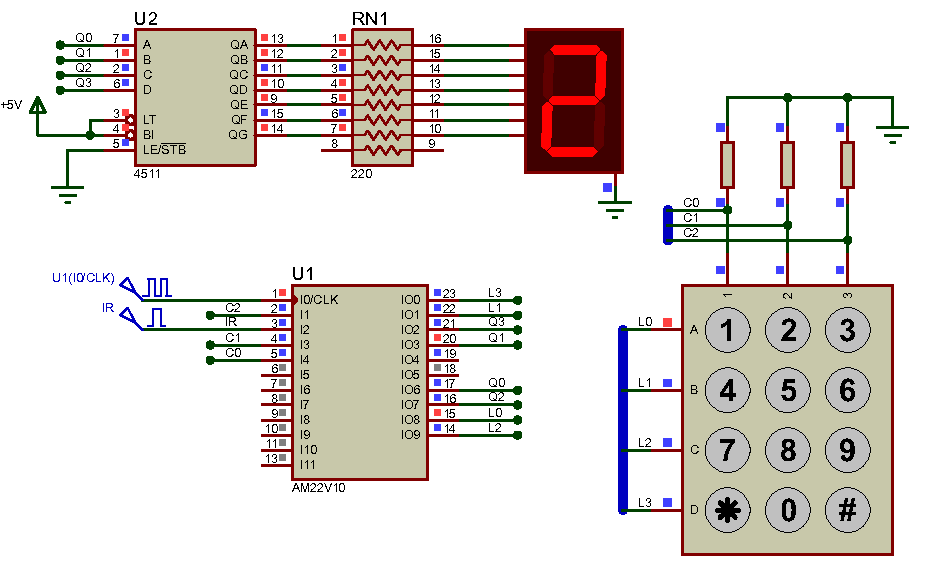
\includegraphics[scale=0.8]{Graphics/VHDL/Practice 5/7-SEG/ANIMATION/F2.PDF}
    }\fi
    
    \caption{Proteus assembly of 3x4 Keypad Control}
    \label{fig:KEYPAD_PROTEUS}
\end{figure}

\clearpage





















